\begin{center}

  \begin{tabular}{rp{16cm}lp{20cm}}%{rl}

  % after \\: \hline or \cline{col1-col2} \cline{col3-col4} ...

  论文地址:& \href{https://arxiv.org/pdf/2010.07922.pdf}{https://arxiv.org/pdf/2010.07922.pdf} \\
  来源:& ICLR, 2021\\
  作者:& Jovana Mitrovic, Brian McWilliams, et al. \\

  %源码:& \href{xxx}{xxx} \\

%  slides:& \href{http://yunshengb.com/wp-content/uploads/2017/03/nips_2018_r2l_workshop_talk.pdf}{{\footnotesize Convolutional Set Matching for Graph Similarity}}\\

  关键词:& \textbf{Self-Supervised learning, Contrastive Learning, Causal} \\

  写于:& \date{2021-03-31}

  \end{tabular}

\end{center}

该论文\cite{mitrovic2021representation}从因果的视角下解释自监督学习,将数据生成过程看成由两个因子控制的过程。并且提出了RELIC(Representation Learning with Invariant Mechanisms),能够学习到尽量与下游任务无关的表征。

\paragraph{问题定义}
$X$表示未标记的数据,$\mathcal{Y} = \{Y_t\}_{t=1}^{T}$表示一系列未知的下游任务。目标就是使用$X$学习到有利于$\mathcal{Y}$的表征。

\paragraph{RELIC}
\begin{figure}[h]
	\centering
	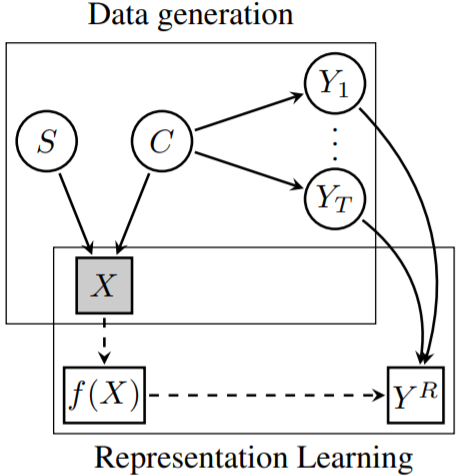
\includegraphics[width=.3\textwidth]{pics/Causal.png}
	\caption{Data Generation in  Causal interpretation}
	\label{fig:causal}
\end{figure}
该论文主要针对的一个问题是:通过自监督学习到的表征尽量与下游任务无关。为了解决这个问题,作者将数据生成看作是有因果关系的,如Fig.\ref{fig:causal}所示。其中S,C分别表示Style和Content。并有三个前提假设:1)数据是由S,C生成的(有点变分推断\cite{kingma2014autoencoding}的味道);2)只有C与下游任务是相关的;3)C和S是不相关的。

在这里,S表示不同的数据增强方式。为了使数据的表则在不同的Style下是与下游任务是无关的,需要满足如下形式:
$$
p^{do(a_i)}(Y^R \:|\: f(X)) = p^{do(a_j)}(Y^R \:|\: f(X))\quad \forall a_i, a_j \in \mathcal{A}
$$
其中$p^{do(a_i)}$表示施加Style $a_i$后的数据分布,$\mathcal{A}$表示数据增强方式集合,即所有的styles。为了在不同的数据增强方式下对下游任务都是无关的,作者还提出了一个正则化项,最终的目标函数如下:
$$
\mathop{\mathbb{E}}\limits_{X} \mathop{\mathbb{E}}\limits_{a_{lk},a_{qt} \sim \mathcal{A} \times \mathcal{A}} \sum_{b \in\{a_{il,a_{qt}}\}} \mathcal{L}_b (Y^R, f(X))\quad s.t.\quad KL(p^{do(a_{lk})}(Y^R \:|\: f(X)), p^{do(a_{qt})}(Y^R \:|\: f(X))) \leq \rho
$$


\paragraph{总结}

\begin{itemize}

	\item 用因果解释自监督学习的过程,并且提出了使表征与下游任务无关的学习目标
	\item 看的不是很懂,还是太菜了\emoji{joy}

\end{itemize}

